\documentclass[11pt]{article}
\usepackage[utf8]{inputenc}
\usepackage[T1]{fontenc}
\usepackage{amsmath}
\usepackage{amssymb}
\usepackage{multicol}
\usepackage{geometry}
\usepackage{tikz}
\usepackage{enumitem}
\usepackage{xcolor}
\usepackage{titlesec}
\usepackage{graphicx}

% Configurações de layout
\geometry{a4paper, left=1cm, right=1cm, top=0.5cm, bottom=1.2cm}
\setlength{\columnseprule}{0.4pt}

% Cores para títulos
\titleformat{\section}{\normalfont\Large\bfseries\color{blue}}{\thesection}{1em}{}
\titleformat{\subsection}{\normalfont\large\bfseries\color{red}}{\thesubsection}{1em}{}

\title{\textcolor{blue}{Terceiro Trimestre: Matemática \\
Medidas de Tendência Central}}
\author{Professor: Jefferson}
\date{}

\begin{document}

\maketitle
\vspace{-1cm}

\begin{center}
\large{Nome: \underline{\hspace{8cm}} \quad Turma: \underline{\hspace{3cm}}}
\end{center}

\begin{multicols}{2}

\section*{Objetivo da Aula}

% CAIXA COLORIDA COM A HABILIDADE
\begin{tikzpicture}
\node[rectangle, 
      fill=purple!15, 
      rounded corners=5pt, 
      inner sep=10pt, 
      draw=purple!60!black, 
      thick,
      drop shadow={opacity=0.3}] (box) 
{
\begin{minipage}{0.75\linewidth}
\justifying
\small
\textbf{(EM13MAT316PE32)} Resolver e elaborar situações problema, em contextos diversos, que envolvam o cálculo e a interpretação das medidas de tendência central (média, moda, mediana) e das medidas de dispersão (amplitude, variância e desvio padrão), com e/ou sem apoio de tecnologias digitais.
\end{minipage}
};
\end{tikzpicture}

\vspace{5mm}

\section*{1. Medidas de Tendência Central}

\subsection*{Média Aritmética ($\bar{x}$)}

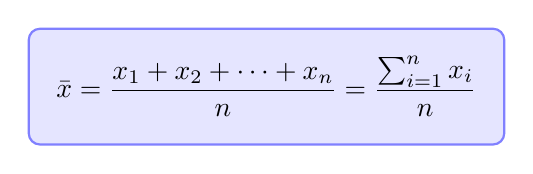
\begin{tikzpicture}
\node[rectangle, fill=blue!10, rounded corners, inner sep=10pt, draw=blue!50, thick] (box) {
$\displaystyle \bar{x} = \frac{x_1 + x_2 + \cdots + x_n}{n} = \frac{\sum_{i=1}^{n} x_i}{n}$
};
\end{tikzpicture}

\vspace{5mm}

\textbf{Onde:}
\begin{itemize}
\item $\textcolor{red}{x_i}$ = cada valor do conjunto
\item $\textcolor{red}{n}$ = número total de valores
\end{itemize}

\subsection*{Exemplo:}
Calcule a média das notas: 7, 8, 6, 9, 5
\[
\bar{x} = \frac{7 + 8 + 6 + 9 + 5}{5} = \frac{35}{5} = 7
\]

\subsection*{Moda (Mo)}

\resizebox{1.0\linewidth}{!}{%
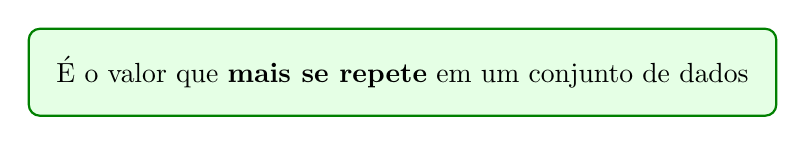
\begin{tikzpicture}
\node[rectangle, fill=green!10, rounded corners, inner sep=10pt, draw=green!50!black, thick] (box) {
É o valor que \textbf{mais se repete} em um conjunto de dados
};
\end{tikzpicture}
    }

\vspace{5mm}

\textbf{Tipos:}
\begin{itemize}
\item \textbf{Amodal}: nenhum valor se repete
\item \textbf{Unimodal}: apenas uma moda
\item \textbf{Bimodal}: duas modas
\item \textbf{Multimodal}: três ou mais modas
\end{itemize}

\subsection*{Exemplo:}
\begin{itemize}
\item Conjunto A: 2, 3, 5, 7, 8 → \textbf{Amodal}
\item Conjunto B: 4, 5, 5, 6, 7 → \textbf{Moda = 5}
\item Conjunto C: 2, 3, 3, 4, 4, 5 → \textbf{Bimodal: 3 e 4}
\end{itemize}

\subsection*{Mediana (Md)}

\resizebox{1.1\linewidth}{!}{%
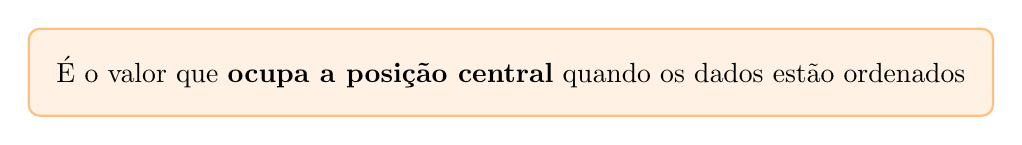
\begin{tikzpicture}
\node[rectangle, fill=orange!10, rounded corners, inner sep=10pt, draw=orange!50, thick] (box) {
É o valor que \textbf{ocupa a posição central} quando os dados estão ordenados
};
\end{tikzpicture}%
}

\vspace{5mm}

\textbf{Como calcular:}
\begin{enumerate}
\item Ordene os dados em ordem crescente
\item Se $n$ é ímpar: $Md =$ valor central
\item Se $n$ é par: $Md =$ média dos dois valores centrais
\end{enumerate}

\subsection*{Exemplo:}
\begin{itemize}
\item Conjunto ímpar: 3, 5, 7, 9, 11 → $Md = 7$
\item Conjunto par: 2, 4, 6, 8, 10, 12 → $Md = \frac{6 + 8}{2} = 7$
\end{itemize}

\section*{2. Exercícios Práticos}

\subsection*{Exercício 1: Cálculo Básico}
Calcule a média, moda e mediana para os seguintes conjuntos de dados:

\begin{enumerate}[label=\alph*)]
\item Notas de matemática: 5, 7, 6, 8, 7, 9, 7, 6, 8, 5
\item Idades: 12, 14, 13, 15, 14, 16, 14, 13
\item Temperaturas (°C): 22, 24, 23, 25, 24, 24, 26
\end{enumerate}

\subsection*{Exercício 2: Análise de Dados}
As alturas (em cm) dos jogadores de um time de vôlei são:
185, 192, 188, 195, 192, 190, 185, 198, 192, 190

\begin{enumerate}[label=\alph*)]
\item Calcule a altura média do time
\item Qual é a moda das alturas?
\item Determine a mediana
\item Quantos jogadores estão acima da altura média?
\end{enumerate}

\subsection*{Exercício 3: Situação Problema}
Em uma pesquisa sobre o número de irmãos dos alunos de uma turma, foram obtidos os seguintes dados:
0, 1, 2, 1, 3, 1, 2, 4, 1, 2, 1, 0, 2, 1, 3

\begin{enumerate}[label=\alph*)]
\item Organize os dados em ordem crescente
\item Calcule a média de irmãos por aluno
\item Qual é a moda?
\item Determine a mediana
\item Que porcentagem dos alunos tem 2 ou mais irmãos?
\end{enumerate}

\subsection*{Exercício 4: Interpretação de Resultados}
As vendas diárias (em R\$) de uma loja durante 10 dias foram:
250, 300, 280, 350, 400, 320, 290, 310, 380, 420

\begin{enumerate}[label=\alph*)]
\item Calcule a venda média diária
\item Qual é a mediana das vendas?
\item Existe moda? Justifique
\item Se a meta de vendas é R\$ 350,00 por dia, em quantos dias a loja atingiu ou superou a meta?
\end{enumerate}

\section*{3. Problemas Desafiadores}

\subsection*{Problema 1: Análise Salarial}
Os salários mensais dos funcionários de uma pequena empresa são:
R\$ 1.200, R\$ 1.500, R\$ 1.800, R\$ 2.000, R\$ 2.000, R\$ 2.200, R\$ 2.500, R\$ 3.000, R\$ 8.000

\begin{enumerate}[label=\alph*)]
\item Calcule a média salarial
\item Determine a mediana
\item Qual é a moda?
\item Qual medida melhor representa o salário típico dos funcionários? Justifique
\item O que a diferença entre média e mediana revela sobre a distribuição salarial?
\end{enumerate}

\subsection*{Problema 2: Comparação de Turmas}
As notas finais de duas turmas em matemática foram:

\begin{itemize}
\item \textbf{Turma A}: 6, 7, 8, 5, 9, 7, 6, 8, 7, 6, 5, 8, 9, 7, 6
\item \textbf{Turma B}: 4, 5, 6, 7, 8, 9, 5, 6, 7, 8, 4, 5, 6, 7, 10
\end{itemize}

\begin{enumerate}[label=\alph*)]
\item Para cada turma, calcule média, moda e mediana
\item Qual turma teve melhor desempenho geral?
\item Compare a distribuição das notas das duas turmas
\item Se a média para aprovação é 6,0, qual turma teve maior porcentagem de aprovados?
\end{enumerate}

\subsection*{Problema 3: Tendência Central e Tomada de Decisão}
Uma empresa está analisando o tempo (em minutos) que seus funcionários levam para completar uma tarefa:

\begin{itemize}
\item \textbf{Grupo X}: 25, 28, 30, 32, 35, 38, 40, 45, 50, 120
\item \textbf{Grupo Y}: 35, 36, 37, 38, 39, 40, 41, 42, 43, 44
\end{itemize}

\begin{enumerate}[label=\alph*)]
\item Para cada grupo, calcule as três medidas de tendência central
\item Qual grupo é mais eficiente? Justifique
\item Qual medida é mais afetada por valores extremos (outliers)?
\item Se você fosse o gerente, qual medida usaria para avaliar o desempenho dos grupos? Por quê?
\end{enumerate}

\section*{4. Questões de Vestibular}

\subsection*{Questão 1 (Adaptada ENEM)}
Em uma escola, as notas de uma prova de matemática foram organizadas na tabela abaixo:

\begin{center}
\begin{tabular}{|c|c|}
\hline
\textbf{Nota} & \textbf{Número de Alunos} \\
\hline
4 & 2 \\
5 & 5 \\
6 & 8 \\
7 & 12 \\
8 & 10 \\
9 & 7 \\
10 & 3 \\
\hline
\end{tabular}
\end{center}

Calcule:
\begin{enumerate}[label=\alph*)]
\item A nota média da turma
\item A moda
\item A mediana
\item A porcentagem de alunos com nota acima da média
\end{enumerate}

\subsection*{Questão 2 (UERJ)}
As idades dos participantes de um curso são: 18, 19, 20, 21, 22, 23, 24, 25, 60.

\begin{enumerate}[label=\alph*)]
\item Calcule a média e a mediana das idades
\item Qual medida representa melhor a idade típica dos participantes? Justifique
\item Se o participante de 60 anos não tivesse feito o curso, como mudariam a média e a mediana?
\end{enumerate}

\end{multicols}

\end{document}
